\pagebreak
\section{Cloud Architektur}

Bei den Cloud Architekturen gibt es genau 3 verschiedene Rollen:
\begin{enumerate}
	\item \textbf{Provider:} bietet Cloud Producte/Lösungen an
	\item \textbf{Konsumenten:} konsumieren Cloud Lösungen
	\item \textbf{Klient:} nehmen Cloud Lösungen (Anwendungen/Daten) in Anspruch
\end{enumerate}

\subsection{Konzeptuelle Sichtweise}

In diesem Abschnitt werden die Architekturen der einzelnen Kategorien von Cloudlösungen beschrieben.

\subsubsection{Konsumenten Sichtweise}

\begin{figure}[H]
    \centering
	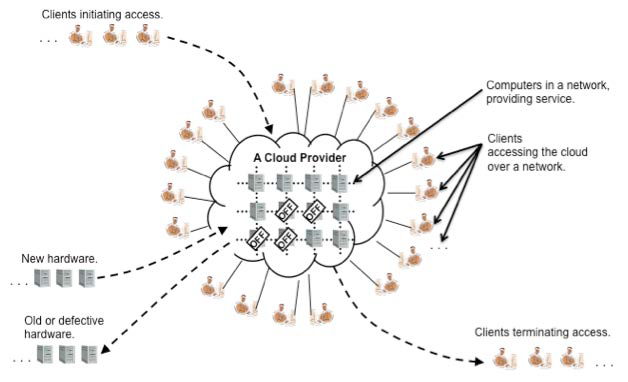
\includegraphics[width=0.4\textwidth]{Images/ConsumerView}
	\caption{Cosumer View \cite{Badger}}
	\label{ConsumerView}
\end{figure}

Um die folgenden Cloud Architekturen zu verstehen, wird 


\subsubsection{Lokale Private Cloud}
\begin{figure}[H]
    \centering
	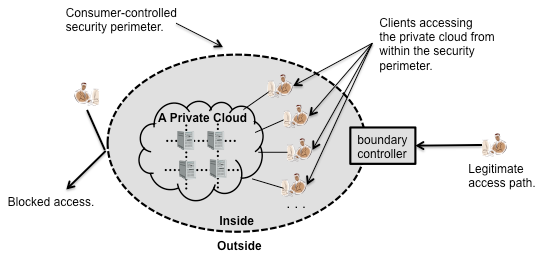
\includegraphics[width=0.4\textwidth]{Images/On-sitePrivateCloud}
	\caption{Private Cloud \cite{Badger}}
	\label{PrivateCloud}
\end{figure}


\subsubsection{Ausgelagerte Private Cloud}
\begin{figure}[H]
    \centering
	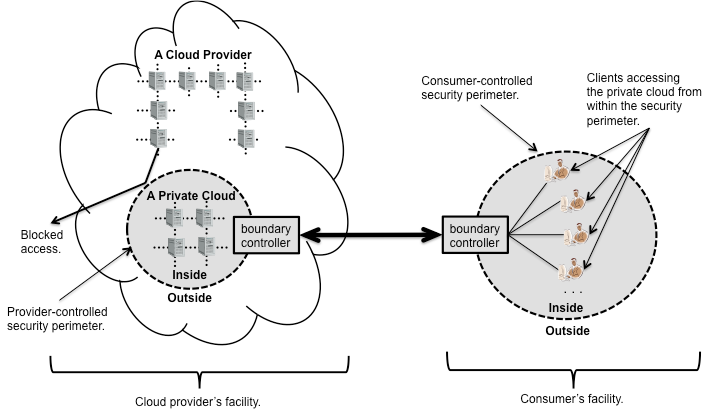
\includegraphics[width=0.4\textwidth]{Images/OutSourcedPrivateCloud}
	\caption{Ausgelagerte Private Cloud \cite{Badger}}
	\label{OutSourcedPrivateCloud}
\end{figure}


\subsubsection{Lokale Community Cloud}
\begin{figure}[H]
    \centering
	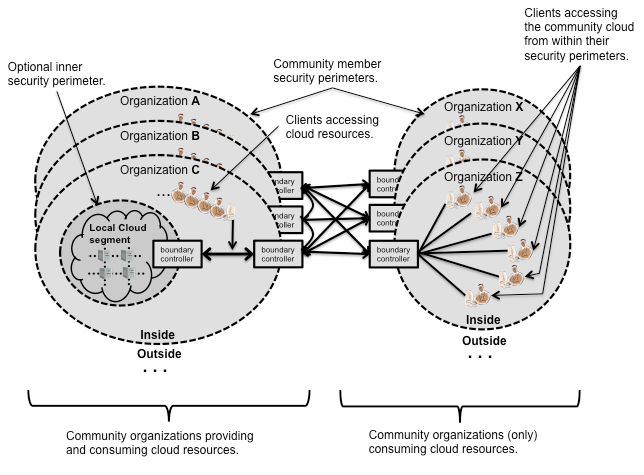
\includegraphics[width=0.4\textwidth]{Images/On-siteCommunityCloud}
	\caption{Lokale Community Cloud \cite{Badger}}
	\label{On-siteCommunityCloud}
\end{figure}



\subsubsection{Ausgelagerte Community Cloud}
\begin{figure}[H]
    \centering
	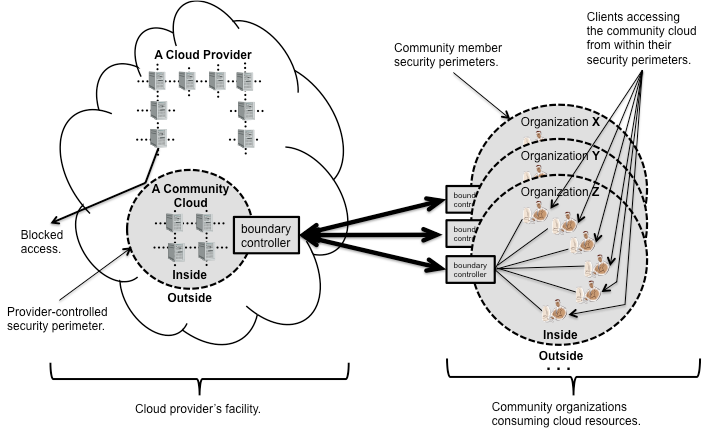
\includegraphics[width=0.4\textwidth]{Images/OutSourcedCommunityCloud}
	\caption{Ausgelagerte Community Cloud \cite{Badger}}
	\label{OutSourcedCommunityCloud}
\end{figure}


\subsubsection{Public Cloud}
\begin{figure}[H]
    \centering
	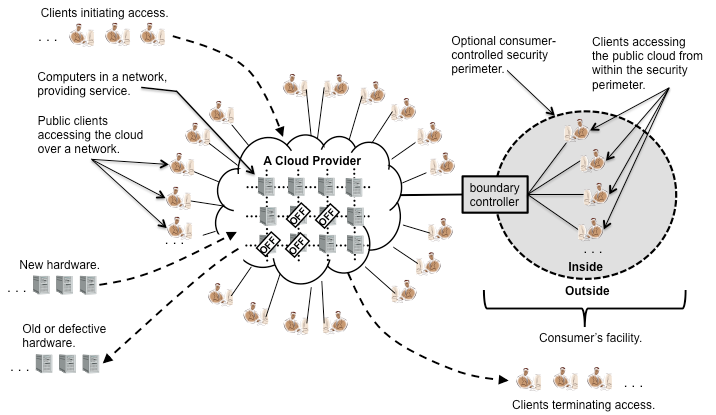
\includegraphics[width=0.4\textwidth]{Images/PublicCloud}
	\caption{Public Cloud \cite{Badger}}
	\label{PublicCloud}
\end{figure}


\subsubsection{Hybrid Cloud}
\begin{figure}[H]
    \centering
	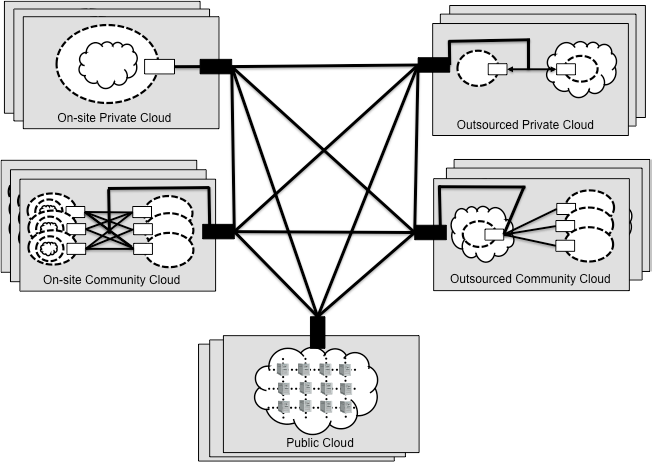
\includegraphics[width=0.4\textwidth]{Images/HybridCloud}
	\caption{Hybrid Cloud \cite{Badger}}
	\label{HybridCloud}
\end{figure}


\subsubsection{SaaS}
\begin{figure}[H]
    \centering
	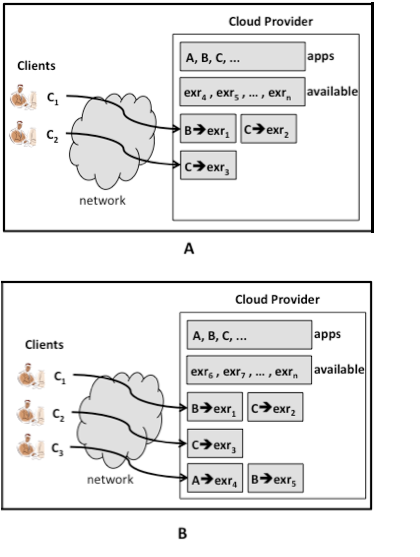
\includegraphics[width=0.4\textwidth]{Images/SaaSInteraction}
	\caption{Hybrid Cloud \cite{Badger}}
	\label{SaaSInteraction}
\end{figure}

\begin{figure}[H]
    \centering
	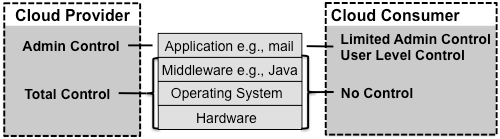
\includegraphics[width=0.4\textwidth]{Images/SaaSControl}
	\caption{Hybrid Cloud \cite{Badger}}
	\label{SaaSControl}
\end{figure}


\begin{figure}[H]
    \centering
	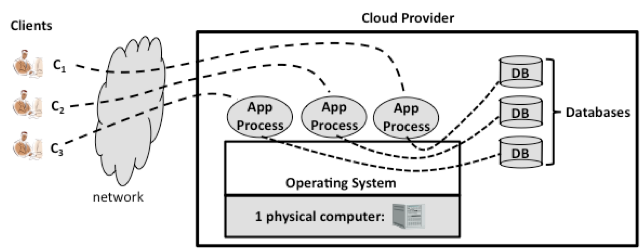
\includegraphics[width=0.4\textwidth]{Images/SaaSM1}
	\caption{Hybrid Cloud \cite{Badger}}
	\label{SaaSM1}
\end{figure}

\begin{figure}[H]
    \centering
	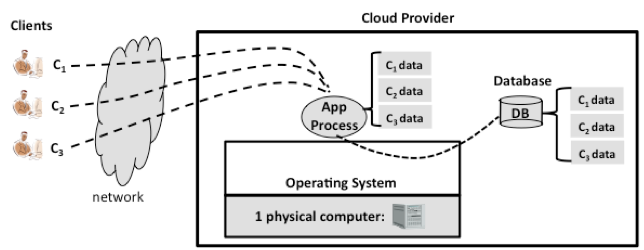
\includegraphics[width=0.4\textwidth]{Images/SaaSM2}
	\caption{Hybrid Cloud \cite{Badger}}
	\label{SaaSM2}
\end{figure}

\subsubsection{Paas}
\begin{figure}[H]
    \centering
	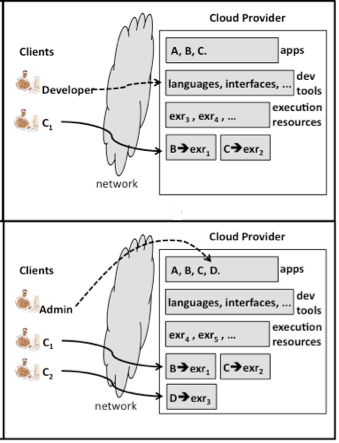
\includegraphics[width=0.4\textwidth]{Images/PaaSInteraction}
	\caption{Hybrid Cloud \cite{Badger}}
	\label{PaaSInteration}
\end{figure}

\begin{figure}[H]
    \centering
	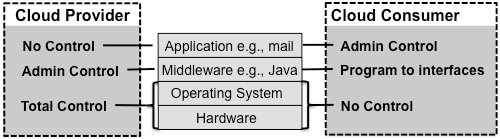
\includegraphics[width=0.4\textwidth]{Images/PaaSControl}
	\caption{Hybrid Cloud \cite{Badger}}
	\label{PaaSControl}
\end{figure}

\subsubsection{IaaS}
\begin{figure}[H]
    \centering
	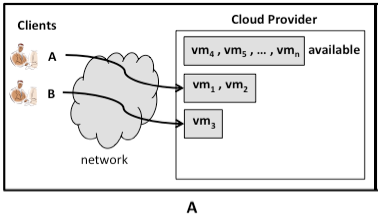
\includegraphics[width=0.4\textwidth]{Images/IaaSInteraction}
	\caption{Hybrid Cloud \cite{Badger}}
	\label{IaaSInteraction}
\end{figure}

\begin{figure}[H]
    \centering
	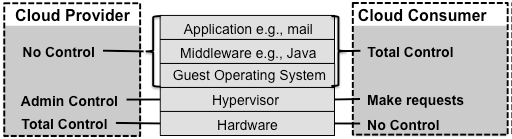
\includegraphics[width=0.4\textwidth]{Images/IaaSControl}
	\caption{Hybrid Cloud \cite{Badger}}
	\label{IaaSControl}
\end{figure}




\pagebreak
\subsection{Logische Sichtweise}
\begin{figure}[H]
    \centering
	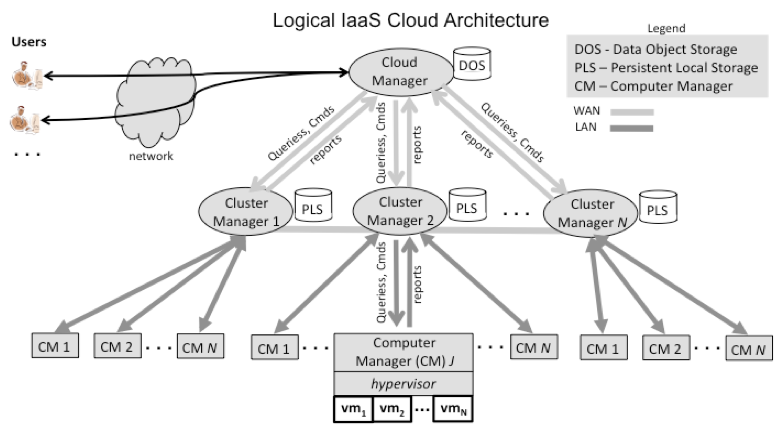
\includegraphics[width=0.4\textwidth]{Images/IaaSLogic}
	\caption{Hybrid Cloud \cite{Badger}}
	\label{IaaSLogic}
\end{figure}

\subsection{Management}
\pagebreak